\begin{savequote}[8cm]
\textlatin{Neque porro quisquam est qui dolorem ipsum quia dolor sit amet, consectetur, adipisci velit...}

There is no one who loves pain itself, who seeks after it and wants to have it, simply because it is pain...
  \qauthor{--- Cicero's \textit{de Finibus Bonorum et Malorum}}
\end{savequote}

\chapter{\label{ch:4-sel}New Techniques in Selection Development} 

The upgrade new detector has enhanced measuring capabilities. 
The granular structure of SFGD enables precise position and $\dedx$ measurements with fast response.
This is especially important for hadrons, as they tend to have much shorter tracks and are conventionally harder to reconstruct in scintillator detectors compared to muons.
As a result, the explored hadronic kinematic phase space is relatively restricted and the reconstructed hadronic variables have relatively large uncertainties.
Since more exclusive event topology such as $\numuccopiop$ allows the measurement of high-level variables like the Transverse Kinematic Imbalance (TKI) variables, which provide invaluable insights on neutrino-nucleus interactions, it is highly desirable to reconstruct hadrons, to measure their kinematic properties as precisely as possible and to explore their phase space as large as possible.
The T2K ND upgrade make possible the implementation of sophisticated techniques from other experiments, like the Elastically Scattered and Contained proton technique~\cite{Lu:2016mjf} that has shown significant improvement in proton momentum reconstruction resolution, and novel techniques implemented for the first time, i.e. the pion trackless reconstruction technique.
The benefits of these techniques will be illustrated based on MC studies and further showcase in data-MC comparisons for both low level variables, such as the single particle kinematic variables and the high level variables, like the Transverse Kinematic Imbalance (TKI) variables and the Centre-of-Momentum (COM) variables. 

\section{New Techniques}
\minitoc
   Two of the most common product hadrons from neutrino-nucleus interaction are protons and pions. 
   The default particle identification and momentum reconstruction have been developed by colleagues at T2K using the Boosted Decision Tree (BDT) algorithm. The BDT algorithm has good performance, but it is still lacking in some aspects.
   For instance, as it uses only single-track information, it cannot effectively distinguish between pions and muons. 
   It could reconstruct proton momentum with an excellent resolution of about $3.5\%$, but it is insufficient for TKI analysis, which is highly sensitive to hadron kinematics. 
   To address these gaps, I have developed and implemented new techniques for both hadrons. 
   For pions, I have invented the pion trackless reconstruction, a novel technique to reconstruct pions without requiring the presence of a reconstructed track, thereby lowering the detection threshold and significantly increasing reconstruction efficiency for low-momentum pions. 
   As for protons, I have adapted the Elastically Scattered and Contained (ESC) protons technique~\cite{Lu:2016mjf} first implemented in MINERvA to create an ESC proton selection in SFGD, leading to a proton sample with excellent momentum resolution. 

   %------------------- ESC ----------------%
  \subsection{ESC proton selection}

    \subsubsection{Working Principles}
    Protons stopping at rest would deposit a large amount of energy, the so-called Bragg Peak, just before it stops.
    These protons tend to have their momenta better constructed as its momentum is more strongly correlated with its range. 
    As shown in Fig.~\ref{fig:andedx2}, protons having energy below $1000$ units has large variances in momentum reconstruction. 
    \begin{figure}[h]
        \centering
        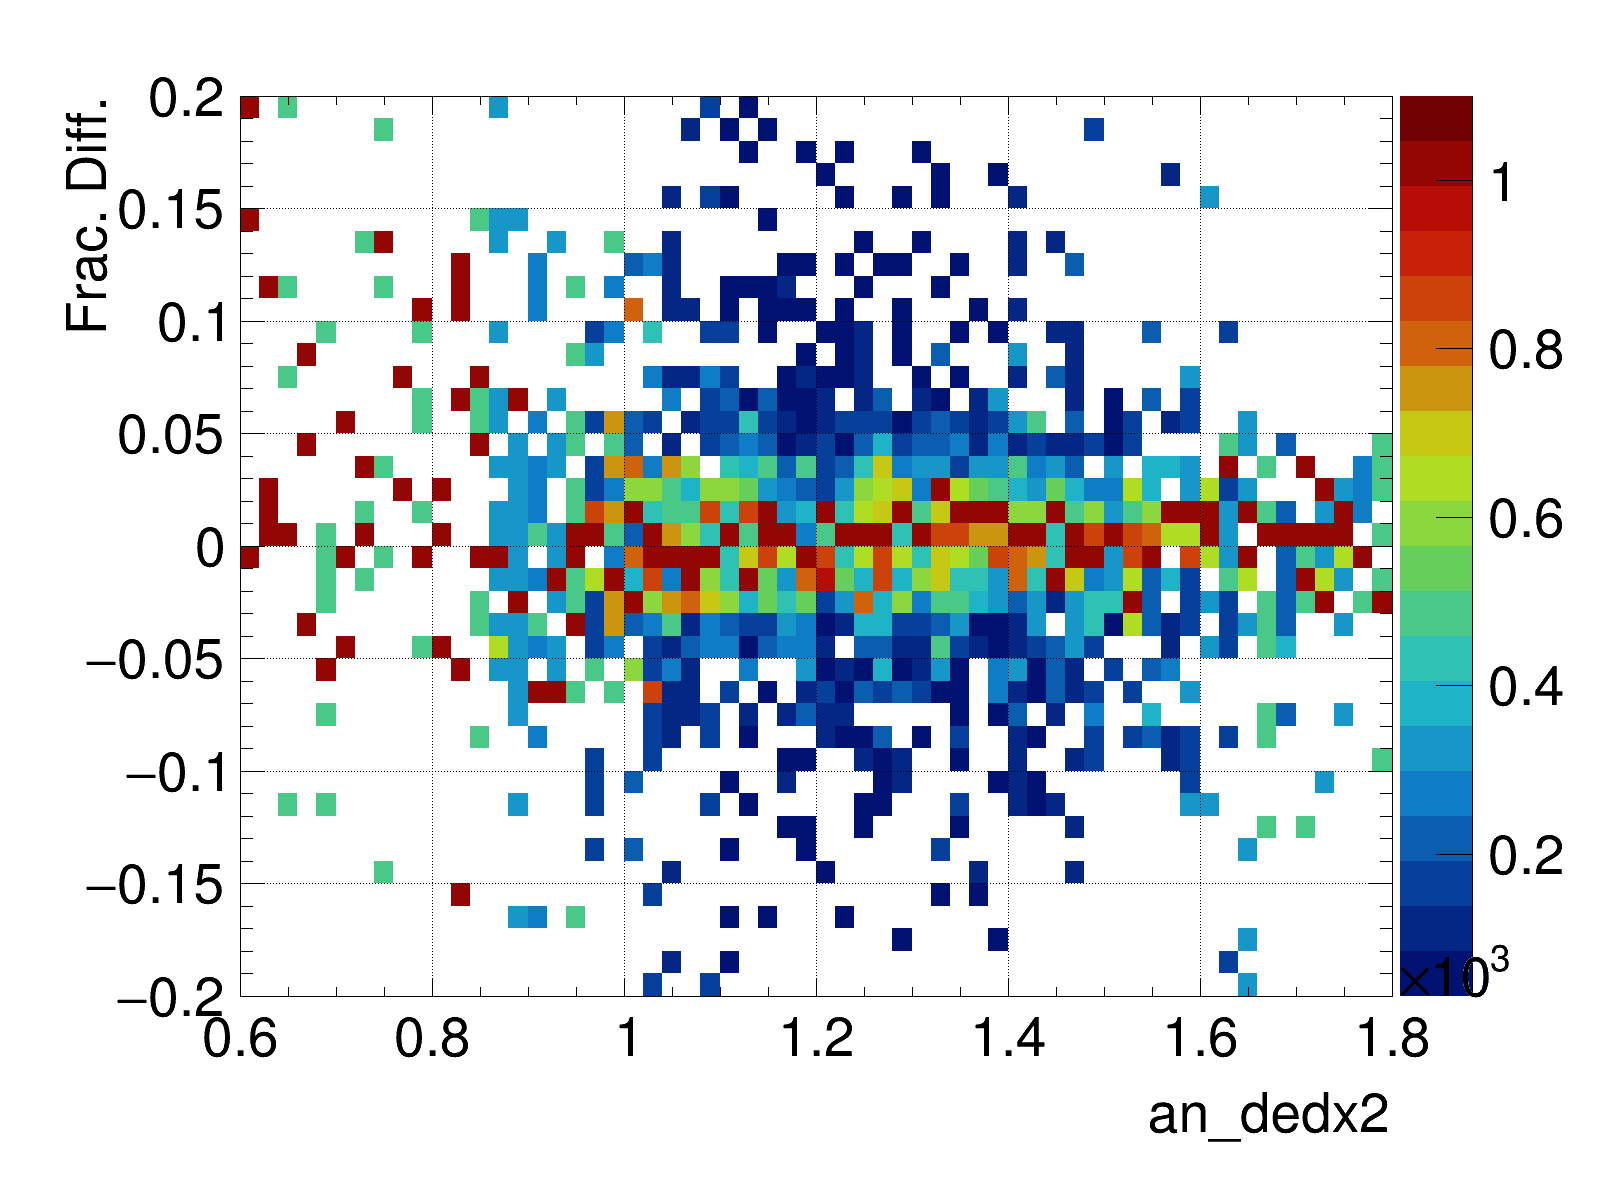
\includegraphics[width=0.5\linewidth]{fig/an_dedx2_colnor_vs_p_pr_res_hist2d_al12_zoom.png}
        \caption{Proton momentum fractional difference against energy deposited at the third last node.}
        \label{fig:andedx2}
    \end{figure}
    Hence, these protons can be selected by placing a lower boundary cut on the energy deposited at the nodes near the end of the reconstructed tracks to have a sample with a high proton momentum resolution.   
    
   \subsubsection{Implementation}
   As the ESC selection is based on $\dedx$ at the end of the proton track, a good reconstuction of $\dedx$ must be obtained first.
   To investigate the proper way of estimatiing $\dedx$, I have simulated multiple particle gun (PGUN) samples with the proton travelling in different directions in the SFGD.
   More specifically, three samples are travelling along the $x$-, $y$- and $z$-axis and five other samples are travelling at $15\degree$, $30\degree$, $45\degree$, $60\degree$ and $75\degree$ to the $x$-axis in the $x$-$z$ plane.
   As the proton direction should not affect its energy deposition, distinct characteristics of $\dedx$ along the proton trajectory can be utilized to validate the quality of the reconstructed $\dedx$.
   Other than the Bragg peak, another distinct feature of $\dedx$ is the minimal ionizing particle (MIP) region, where the particle at high momentum traverses the scintillator despositing the minimal amount of energy. 
   Hence, the $\dedx$ remains at a relatively constant value for all such particles.
   When the $\dedx$ at the end of the proton tracks are plotted, besides the Bragg peak at large $\dedx$, corresponding to protons stopping to rest, there should be another peak at smaller $\dedx$, corresponding protons that undergo secondary interactions and thus are stopped prematurely when it still possesses high momentum.

   The first attempt is to use the smoothed energy directly. 
   Fig.~\ref{fig:dedx-pgun-smoothed} plots energy deposit for the last third to sixth nodes for all PGUN samples travelling at different angles.
   It is reassuring to indeed observe the two peaks, the MIP peak and the Bragg peak, as hypothesized. 
   FIG-PGUN-DEDX-SMOOTH-bfANGNORM
   However, there are still some discrepancies. 
   The MIP peaks are close to each other, but their positions differ noticeably from each other.
   This is due to the different grouping of Hits into Nodes for protons travelling in different directions.
   The different number of Hits in a Nodes lead to different distances between nodes, so using the energy deposited per Node as an estimation of $\dedx$ is not strictly valid anymore.
   To account for the different propagation directions, I divided the energy by the sine of the angle of the trajectory made with the $z$-axis.
   The angle-normalized energy is plotted in Fig.~\ref{fig:dedx-pgun-angnorm}, which demonstrates that the angle-normalization step has achieved its goal - all MIP peaks have the same position.

   FIG-PGUN-DEDX-SMOOTH-afANGNORM

   Hence, the angle-normalized energy can serve as a good reconstruction of $\dedx$ for the ESC selection.
   To determine the suitable threshold $\dedx$ values without biasing the analysis with any underlying information in the signal sample, a stopping proton control sample is used.
   The stopping proton control sample has been developed by a colleague, which aims to select protons traversing one of the two HATs and stopping in SFGD. 
   For these stopping protons, their momenta can be reconstucted independently from HAT and SFGD.
   As momentum reconstruction in HAT (TPC) has high resolution and is well understood, the fractional difference between the reconstructed momenta in HAT and in SFGD for the same track is plotted against the angle-normalized energy to extract the range of $\dedx$ values that possess good momentum reconstruction in SFGD.
   For example, as shown in Fig.~\ref{fig:angnorm-dedx0}, a cut at xxxx should be placed.
   FIG-ANGNORM-dedx0
   FIG-ANGNORM-dedx1
   FIG-ANGNORM-dedx2
   FIG-ANGNORM-dedx3
   FIG-ANGNORM-dedx4
   FIG-ANGNORM-dedx5
   Hence, the respective thresholds for the last 6 nodes are xxx,xxx,xxx,xxx,xxx, and xxx, respectively.

   Furthermore, based on distributions of angle-normalized energy for the last 6 nodes, the average Bragg peak profile can be obtained by fitting the peaks of the distributions.
    The angle-normalized energy for the last 6 nodes for each track can then be compared with this average profile by a $\chi^2$,
    \begin{equation}
     \chi^2 = \Sum^6_1 \frac{(\dedx_i - \overline{\dedx_i})^2}{\overline{\dedx_i}}
    \end{equation}
    A proton coming to rest should have a similar profile, so an upper cut on $\chi^2$ could further select protons with good momentum resolution. 
    Similar to the determination of the threshold for the individual $\dedx$, the momenta fractional difference is plotted against $\chi^2$ as shown in Fig.~\ref{fig:esc-mom-res-chi2}.
    FIG-ESC-MOM-RES-CHI2
    The upper cut on $\chi^2$ is implemented as xxx.

    %------------------- pion TL ----------------%
    \subsection{Pion Trackless Reconstruction}
       As briefly elaborated in Sec.~\ref{sec:t2k-sw}, in SFGD, particle identification and momentum reconstruction are only performed on reconstructed tracks, which has a minimum length of about $30.0$~mm. 
       Hence, low-momentum particles, which travel only a short distance, could not be reconstructed at all. 
       When these low-momentum pions are not reconstructed, these $\ccopi$ events would then be misidentified as $\cczpi$ events, both decreasing the signal for the $\ccopi$ samples and increasing the background for the $\cczpi$ sample. 
       Thus, it would be highly beneficial if we could reconstruct these pions, and the pion trackless reconstruction technique I develop can address this gap perfectly. 

       \subsubsection{Working Principles}
         The trackless technique is an extension and sophistication of previous methods. 
         It was first tried in MINER$\nu$A\cite{MINERVAPOSTER} and in the Fine Grain Detectors of ND280\cite{T2KPOSTER}. 
         In the former, at least a reconstructed cluster is required to be identified as a pion candidate. 
         The latter indeed contains a prototype of the trackless reconstruction, but it is mixed with other pion reconstruction methods and its potential is not fully explored. 
    
         There are two key points of this reconstruction technique based on the pion decay chain, $\pi \rightarrow \mu \rightarrow e$.
         Firstly, the delayed signal of the grandchild, the Michel Electron (ME), is much longer than the time scale of other processes, such as $\piz$ decay.
         Hence, the presence of the primary pion can be inferred by the presence of a delayed signal in the SFGD.
         Secondly, the pion decay, $\pi \rightarrow \mu + \nu$, is a two-body process, the kinematics of the daughters can be completely determined by energy-momentum conservation, 
         When a pion decays at rest, the daughter muon will only move about $0.12~\textrm{cm}$. Hence, the starting point of the ME is a good estimation of the ending point of the pion.
         The pion momentum can then be reconstructed by range based on the distance between the primary neutrino interaction vertex and the ME starting point. 
         A relation between the pion momentum, via its kinetic energy, and its range is obtained from an empirical fit using a PGUN sample, as shown in shown in \figref{fig:fit}.
          The PGUN sample starts from the centre of SFGD and progates isotropically.
          It has a sample size of $500,000$ with a kinetic energy uniformly distributed between $20~\mev$ and $200~\mev$.
          The $\log10$ of the true kinetic energy is plotted against the true pion length as shown in Fig.~\ref{fig:pi-mombr-fit}.
          A fourth order polynomial is fitted to the central region of the plots, where the fitted line matches the data point well.

           \begin{figure}[h]
              \centering
              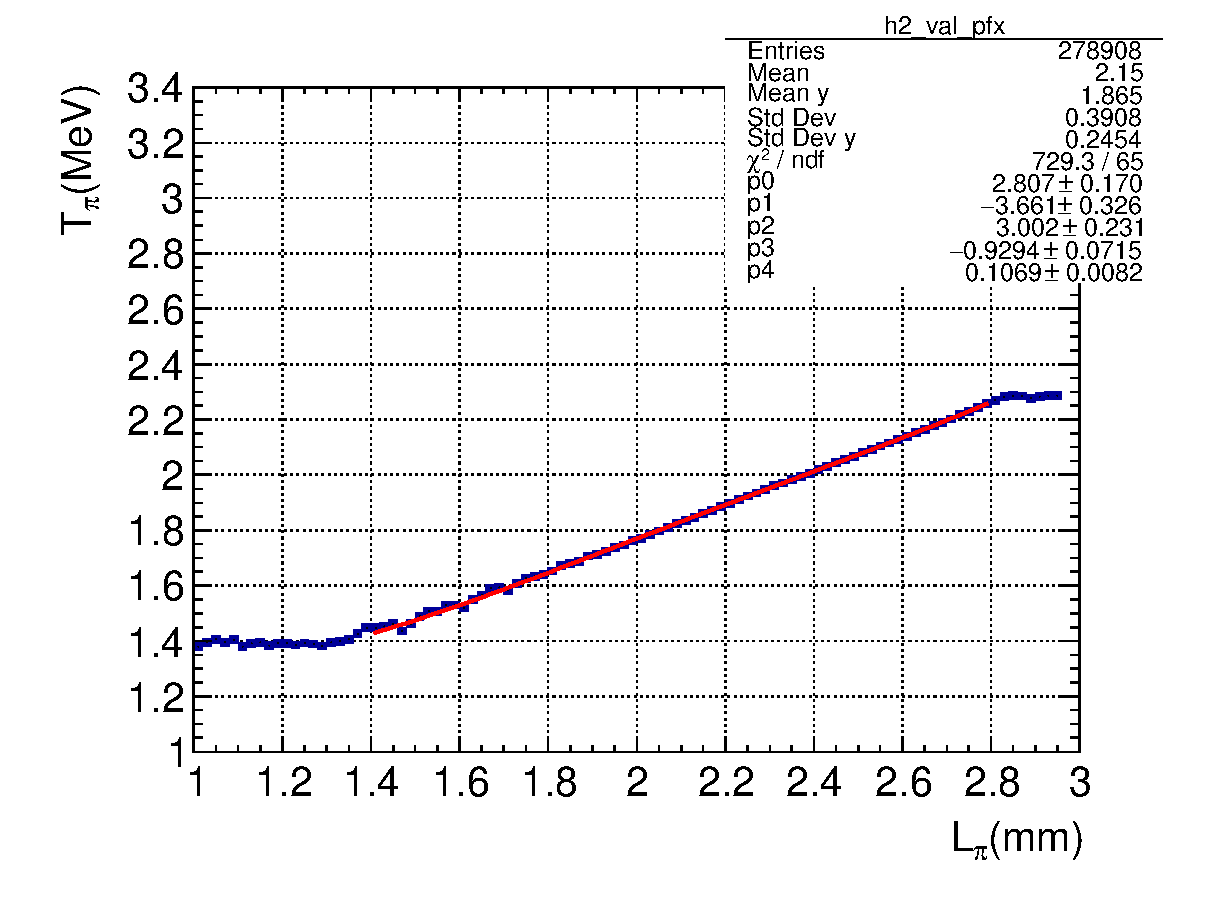
\includegraphics[width=\sgfidwid\textwidth]{figures/pi_len_pi_len_vs_pi_ke_hist2d_al0_true_nokink.eps} 
              \caption{A degree 4 polynomial fit of $\log_{10}{T_\pi}$ against $\log_{10}{L_\pi}$, where $T_\pi$ and $L_\pi$ are the kinetic energy and the range of the pion respectively. The $p_i$'s are the corresponding coefficients of the term of order $i$. The fit is satisfactory considering the close to 1 (\mccorrect{NOT TRUE}) $\chi^2/ndf$ value. }
              \label{fig:fit}
           \end{figure}

        \subsubsection{Implementation}
            The pion trackless reconstruction is part of my $\numuccopi$ selection, which is based on the existing $\numucc$-inclusive selection. Hence, it is best to elaborate the trackless technique in the context of the $\numuccopi$ selection. 
        
            The $\numucc$-inclusive selection has identified the primary vertex position and the primary muon, which already provides the trackless reconstruction with a good approximation of the pion starting point. The following steps are implemented to identify the suitable ME and reconstruct the pion momentum in the $\numuccopi$ selection. 

            \begin{itemize}
                \item Step 0 - \textbf{$\numucc$-inclusive selection.}
                \item Step 1 - \textbf{Find suitable ME candidates.} 
                \item Step 2 - \textbf{One trackless pion cut.}
                \item Step 3 - \textbf{Kink cut.}
                \item Step 4 - \textbf{Background reduction.}
            \end{itemize}
        
            \textbf{Find suitable ME candidates.} - Loop through all delayed reconstructed objects that have more than 1 hit, if it is $30.0~\textrm{ns}$ after the primary vertex time, save it as a potential ME candidate. 
            However, it is common that the ME could trigger a shower, leading to more delayed reconstructed objects. 
            To distinguish the ME from these secondary delayed objects, a technique called the "prompt energy" was used by MINERvA~\cite{Zhang2016}. 
            Prompt energy is the energy deposited by the short muon and the short pion. 
            Even though these particles might have too low energy to leave a reconstruct-able track, they would still deposit energy, which is much early than the onset of ME. 
            Hence, looping through the cubes $30.0~\textrm{mm}$ around the two ends of an ME candidate to observe if there is energy deposited $30.0~\textrm{ns}$ before identifying the proper ME candidate. 
            Moreover, if the primary muon is contained in SFGD, it would also decay to give an ME, which is indistinguishable from a pion ME by just looking at the time delay. 
            Hence, an additional check is added to exclude ME candidates near the end of the identified primary muon. 
        
            \textbf{One trackless pion cut} - Select events that have one and only one proper ME candidate.
        
            \textbf{Kink cut} - As the trackless reconstruction does not require the ME to be near a primary track, it cannot distinguish pions travelling straight from the primary interaction until decaying at rest from those that have undergone a deflection and then decayed at rest. 
            Events with a deflected pion should be rejected as the momentum-by-range reconstruction works only for particles without secondary interaction. 
            Hence, events with an ME connected to any non-primary tracks would be rejected.
        
            \textbf{Background reduction} - Several background reduction steps are implemented, for example, an existing $\pi^0$ rejection developed by Colleagues at T2K.
            However, they are insufficient as shown by the considerable portion of CC-other backgrounds in Fig.~\ref{fig:tlpi-bf-trknumcut}.
            FIG-TLPI-BF-trknumcut
            Hence, based on logical understanding of different event topologies, I developed a series of track number cuts and a new idea, called the track family tree.
            
            An event topology resembles a family tree sideway. 
            The first generation contains the primary tracks.
            The second generation are tracks connecting to the end of the primary tracks.
            The family tree tracing step loops through all reconstructed tracks to form the family tree starting from the primary vertex.
            One useful variable is the number of generations.
            A $\numuccopi$ event should not contain a large number of generations as the primary pion can have an ME attached to its end, but there is no shower or multiple scattering.
            Hence, the number of generation is required to be smaller than $3$.
            Another associated variable is the number of lone tracks, which are not connected to any tracks in the family tree. 
            A clean $\numuccopi$ event should have a limited number of lone tracks, which could be due to noise, or low energy scattering of the ME, which leads to clusters isolated from the ME track. 
            More details of the other track number cuts are provided in Appendix.~\ref{sec:app-tlpi-trknumcut}
        
            For the events passing all the selection steps, the presence of a primary pion is implied by the existence of a proper ME candidate, and its momentum is reconstructed by range. 


    \subsection{Development of stopping pion control sample}
          Conventionally, selections will be used for cross section analysis, which requires a sufficient portion of all detector systematics to be properly evaluated.
          However, due to time constraint, this is unlikely to happen within the time frame of my doctoral study. 
          Hence, only preliminary data-MC comparisons are possible.
          Nontheless, as systematics evaluation is an important ingredient of cross section analysis, which is crucial for improving our understanding of neutrino-nucleus interactions, I implemented the propagation of the systematics of the momentum-by-range reconstruction for pions tagged by ME.
          To evaluate this systematic, I developed the stopping pion control sample with the following steps:
          \begin{enumerate}
          \item Find all tracks that contain an SFGD segment and segments in the other sub-detectors.
          \item Check that one end of this track is stopped in SFGD.
          \item Check the PID of this track provided by the other sub-detectors, i.e. HAT or TPC.
          \item Check that there are no other (except ME) near the track end in SFGD.
          \item A final cut requiring the presence of an ME near the track end in SFGD.
          \item Keep only the event with a single stopping pion candidate.
          \end{enumerate}
          The preliminary result suggests that the control sample consists predorminantly of tracks passing HAT and stopping in SFGD.
          As the current PID in HAT is not fully developed, I investigated further the impact of the log likelihood on pion PID.
          I discovered that the previous cuts need to be made more stringent to achieve a high purity.

          FIG- HAT LLH cuts

          This leads to a sample with over $90\%$ purity as shown in Fig.~\ref{fig:sppi-pur}.
          FIG- SPPI PUR.

           
    
    

\section{MC studies and Comparisons with Data}
     Improvement brought by the implementation of new techniques is best illustrated within the respective selection.

     \subsection{$\numucczpiop$-ESC}

   The lower boundary cut on $\dedx$ and the $\chi^2$ cut are implemented as an extra step on the existing $\numuccopiop$ sample, where the $p$ stands for proton.
   This selection leads to an improvement in proton momentum resolution of about $50\%$ while decreasing the efficiency by about $2/3$, as shown in Fig.~\ref{fig:pprESC-res}.   
   The drop of efficiency might seem drastic, but it proves to be necessary for the TKI analysis, as shown later in Sec.~\ref{sec:do-TKI}. The ESC selection leads to significant improvement to the TKI variables evaluation. 

   \begin{figure}[t]
      \centering
      \begin{subfigure}{0.45\textwidth}
           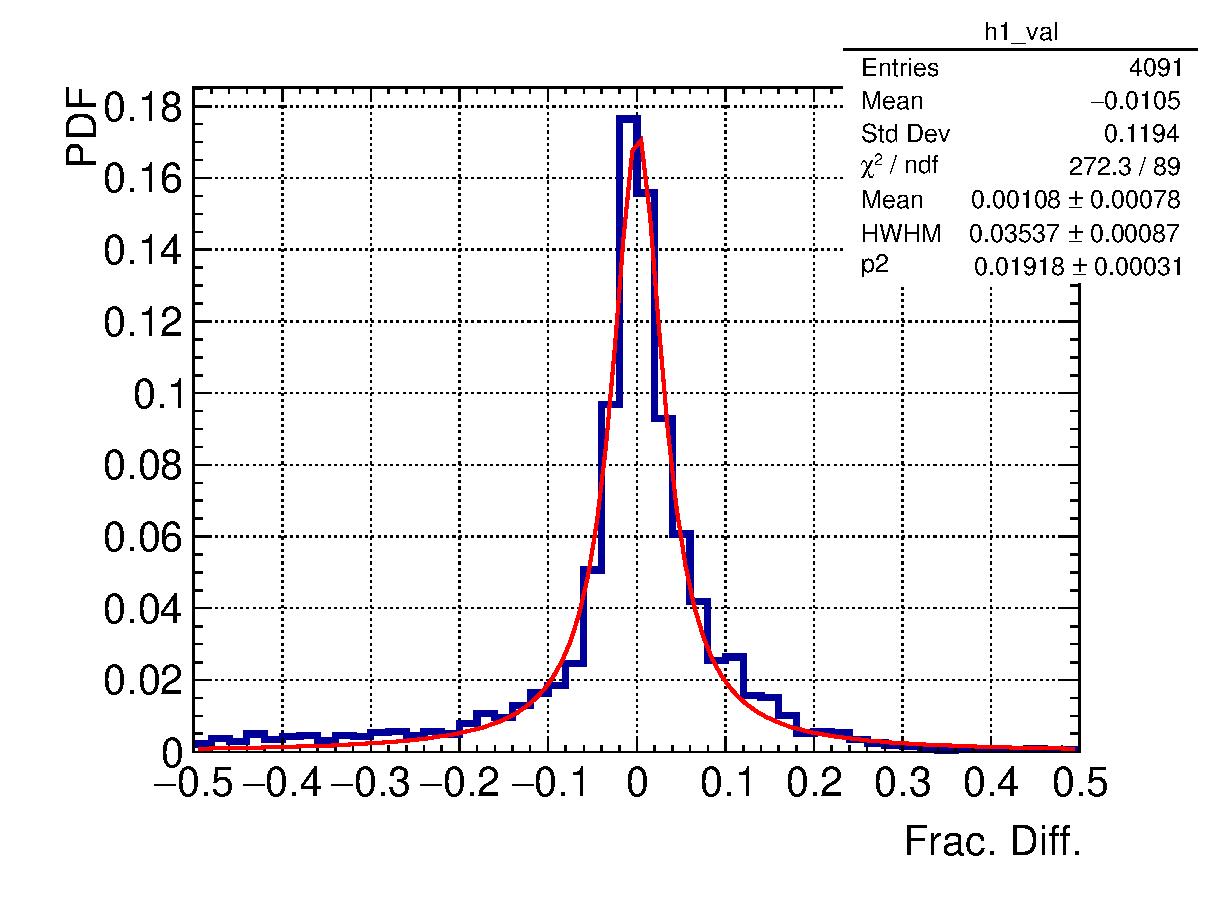
\includegraphics[width=\textwidth]{fig/p_pr_res_pdf_al13_zoom.eps}
           \caption{Momentum resolution before ESC selection.}
           \label{fig:ppr-res-bfESC}
      \end{subfigure}
      \begin{subfigure}{0.45\textwidth}
           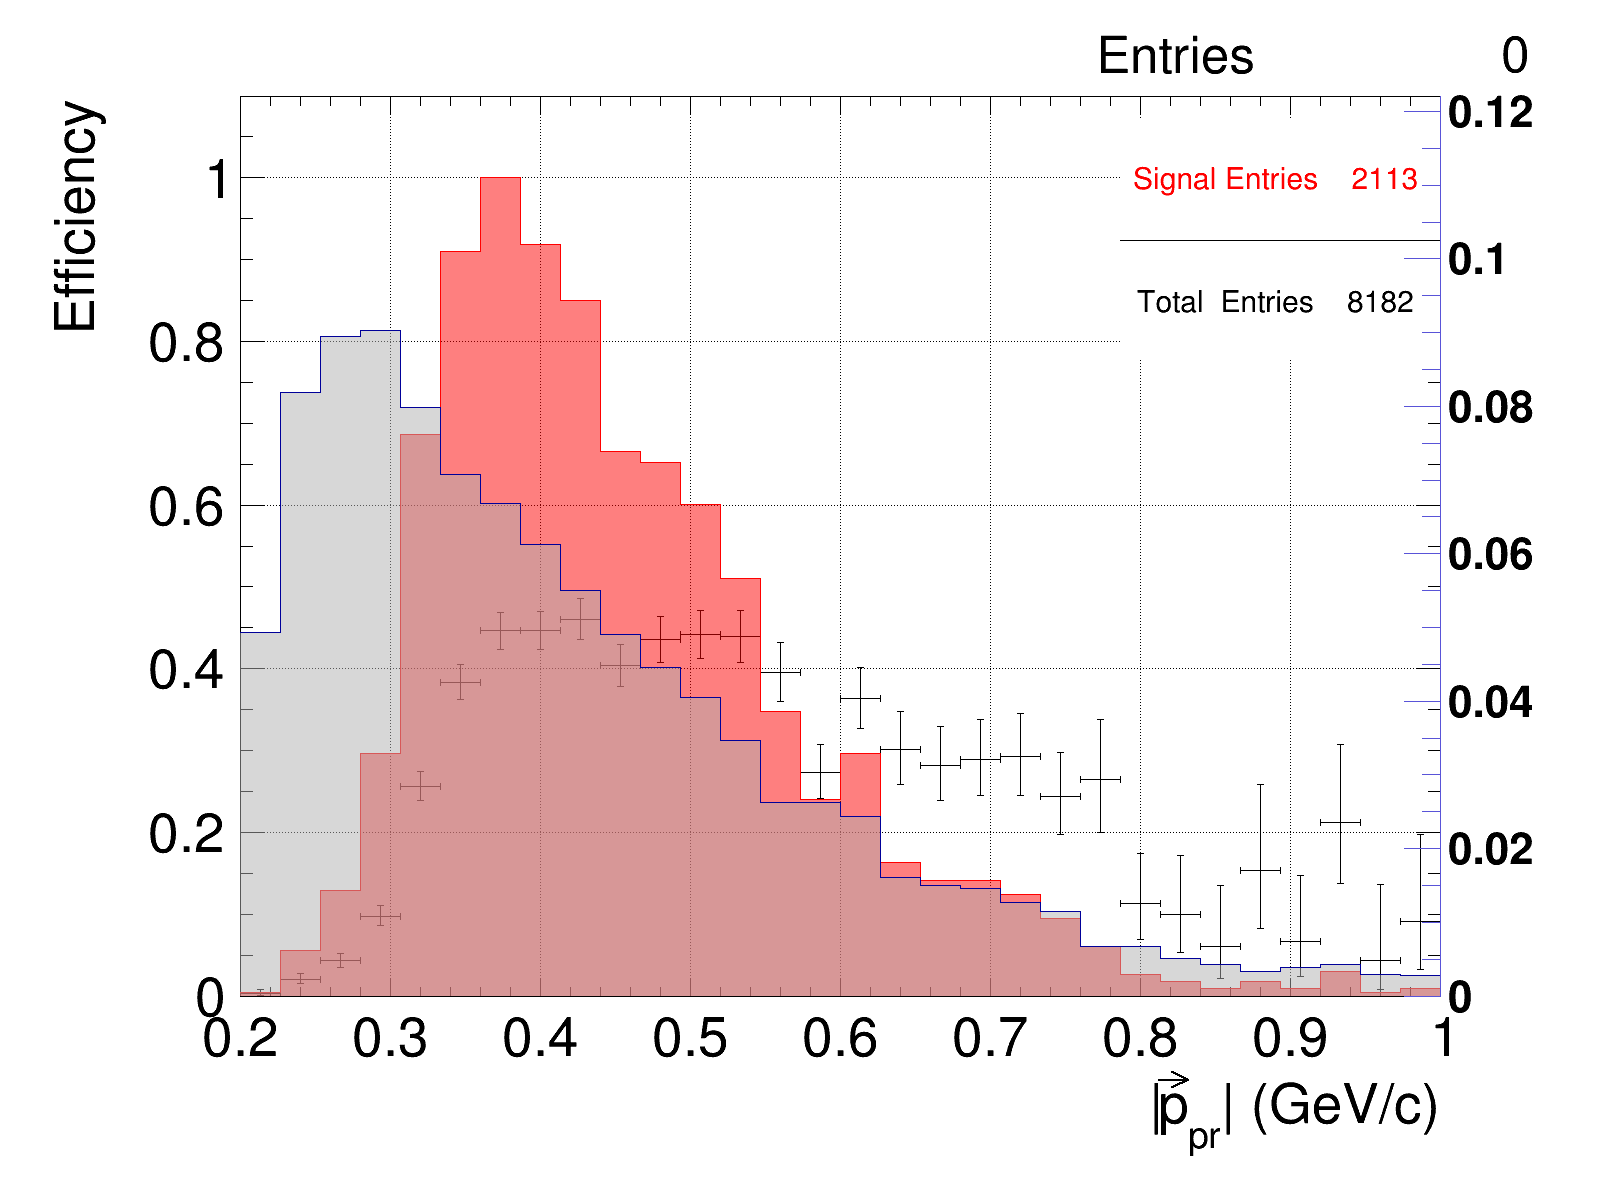
\includegraphics[width=\textwidth]{fig/p_pr_eff_al13.png}
           \caption{Selection efficiency before ESC selection.}
           \label{fig:ppr-eff-bfESC}
      \end{subfigure}
      \\
      \begin{subfigure}{0.45\textwidth}
           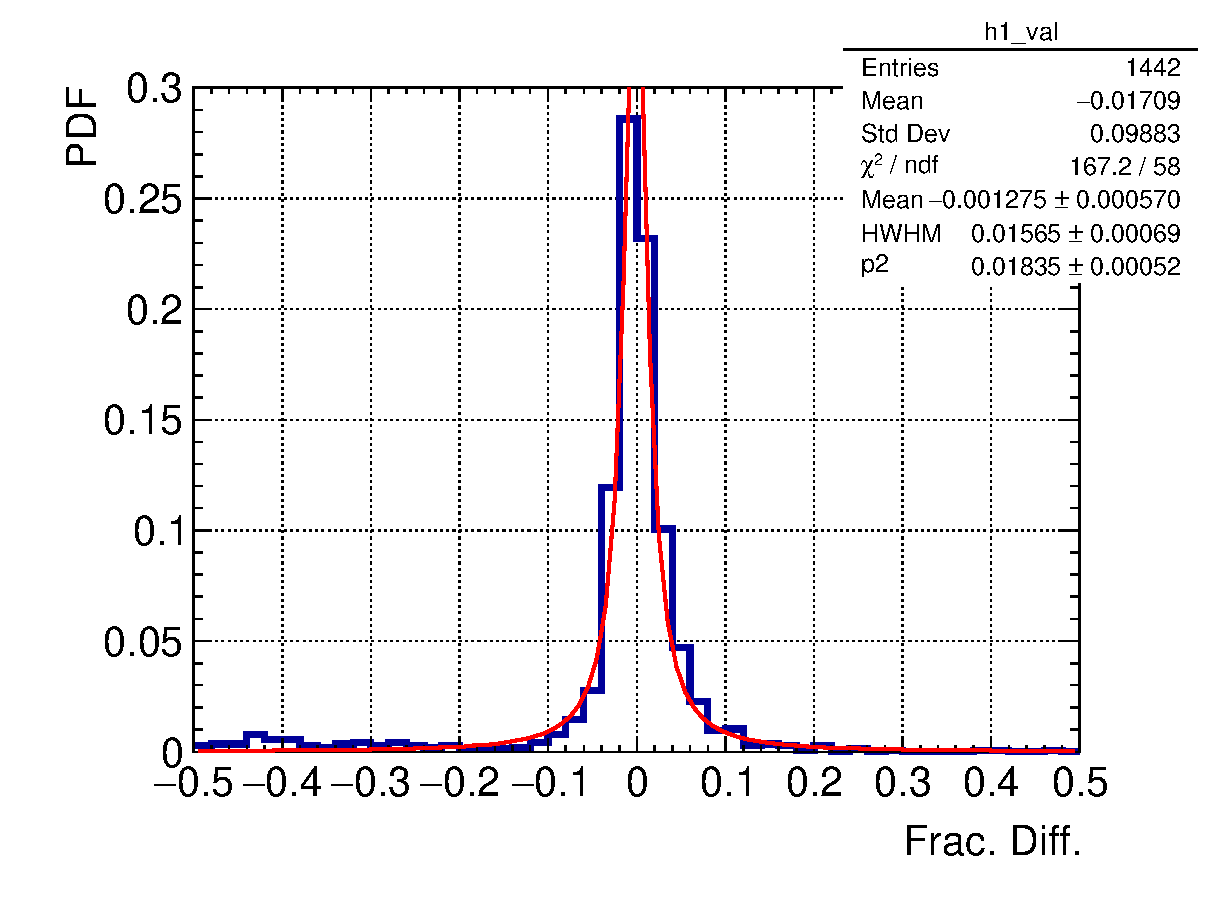
\includegraphics[width=\textwidth]{fig/p_pr_res_pdf_al14_zoom.eps}
           \caption{Momentum resolution after ESC selection.}
           \label{fig:ppr-res-afESC}
      \end{subfigure}
      \begin{subfigure}{0.45\textwidth}
           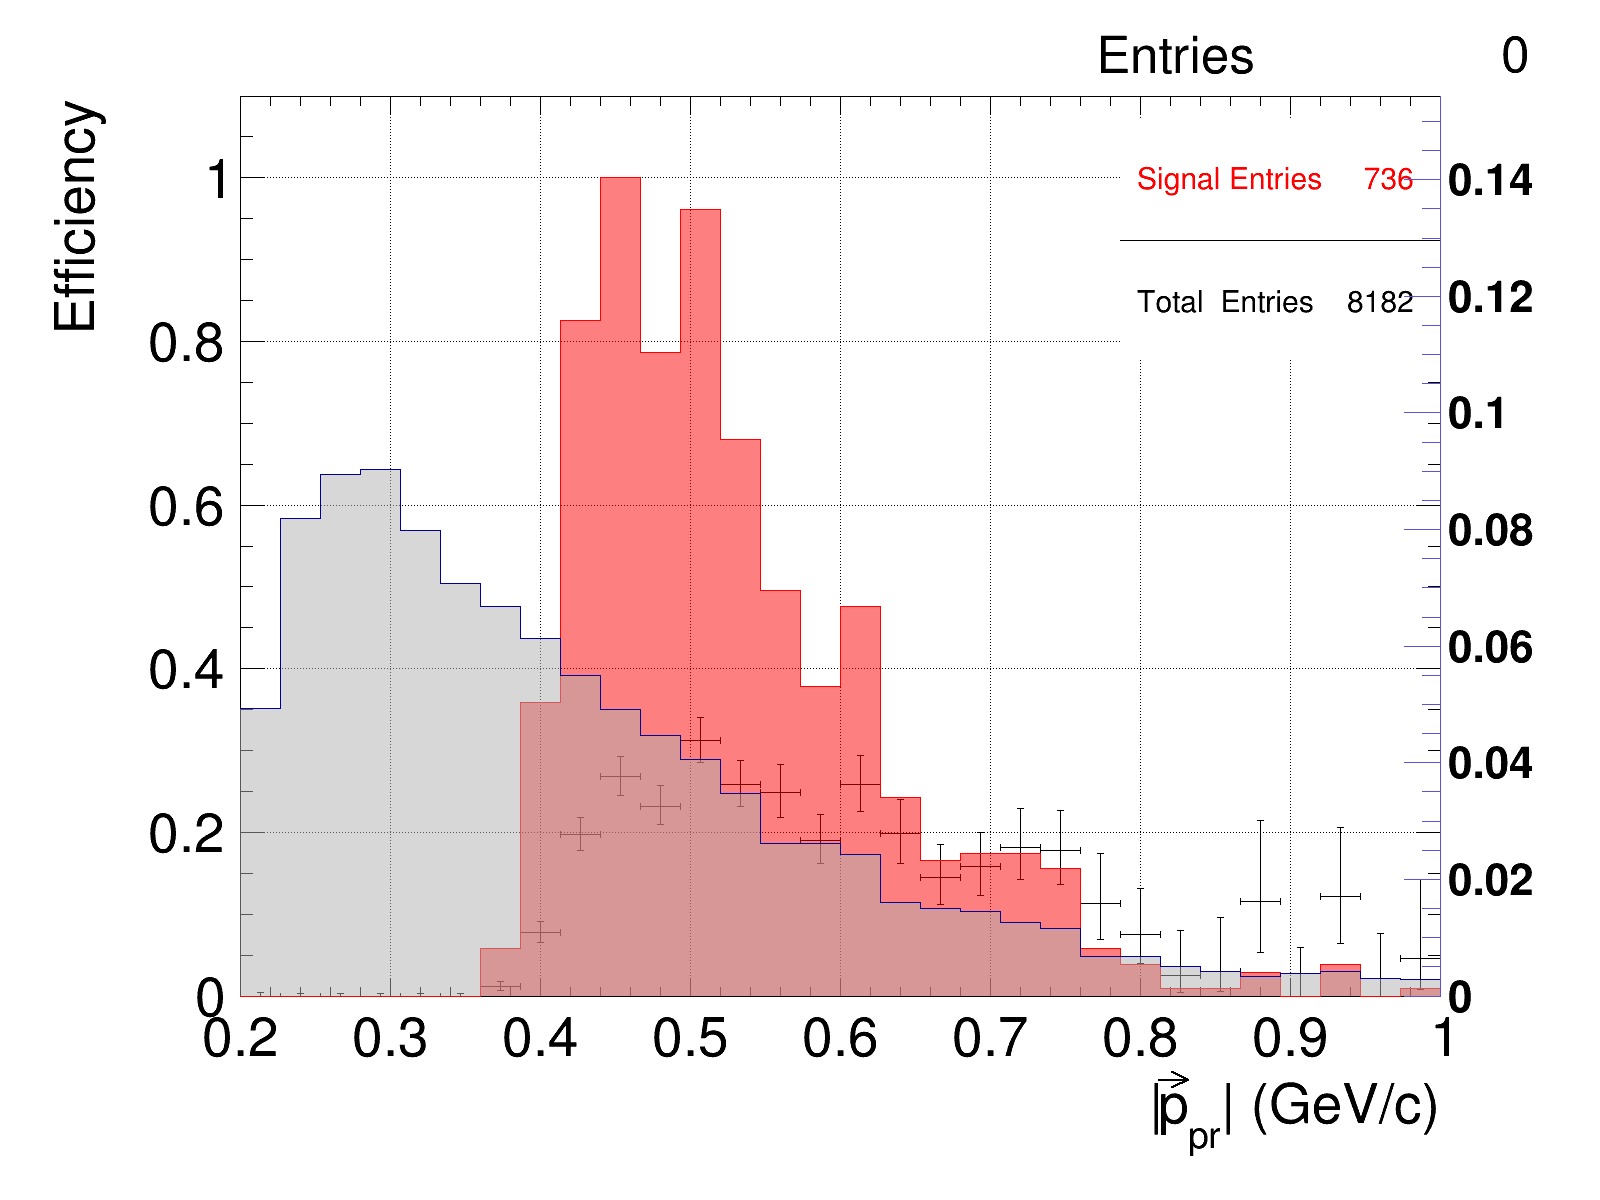
\includegraphics[width=\textwidth]{fig/p_pr_eff_al14.png}
           \caption{Selection efficiency after ESC selection.}
           \label{fig:ppr-eff-afESC}
      \end{subfigure}
      \caption{Proton ESC selection results. The grey histograms are the true probability distribution, while the pink ones are those that get reconstructed. }
      \label{fig:pprESC-res}
   \end{figure}

    
        \subsubsection{Results}
           The results of the $\numuccopi$ selection using the trackless pion technique are summarised in Fig.~\ref{fig:piTLres}.
           As shown in Fig,~\ref{fig:ppi-stack}, the trackless selection has achieved the set goal - reconstructing low momentum pions. 
           There are a considerable number of events with a pion below $100~\mevc$, which correspond to a track of about $50~\textrm{mm}$. 
           Moreover, pions below $80~\mevc$ have also been reconstructed, which travels about $30~\textrm{mm}$ and cannot be reconstructed as a track. 
           Furthermore, the momentum-by-range calculation has achieved an excellent resolution at about $2\%$, as shown in $\ref{fig:ppi-res}$.
           More encouragingly, the overall efficiencies are still relatively high. 
           The step-by-step efficiencies with respect to each step is shown in Fig.~\ref{fig:tl-accum-eff}. 
           The signal definition used in the calculation is to have one true muon that has travelled to the vertical TPC and one true pion that is contained in SFGD. 
           Steps 1 to 7 are the $\numucc$-inclusive selection. 
           The large drop in efficiency in Step 8 is expected as it requires exactly one pion reconstructed tracklessly. 
           All pions undergoing secondary interactions except deflection cannot be reconstructed via this method. 
           Hence, the relative efficiency of $0.37/0.66\approx56\%$ is considerably high. 
           The further significant drop in efficiency comes with the next step, the kink cut, which is a reasonable as a considerable portion of pions undergo deflection. 
           The subsequent drops are graduate cuts to remove backgrounds, which leads to a high purity of $\numuccopi$ as shown in Fig.~\ref{fig:ppi-stack}.

           \begin{figure}[t]
               \centering
               \begin{subfigure}{0.3\textwidth}
                    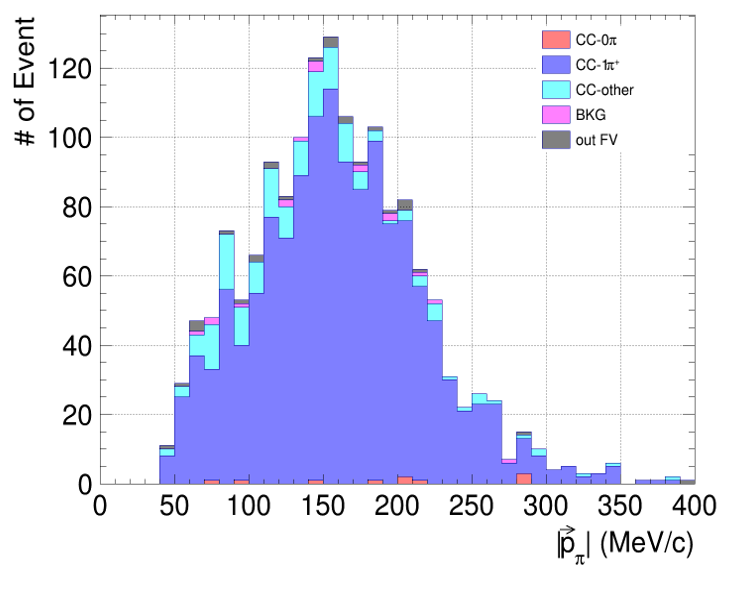
\includegraphics[width=\textwidth]{fig/ppi_stack.png}
                    \caption{Momentum distribution.}
                    \label{fig:ppi-stack}
               \end{subfigure}
               \begin{subfigure}{0.3\textwidth}
                    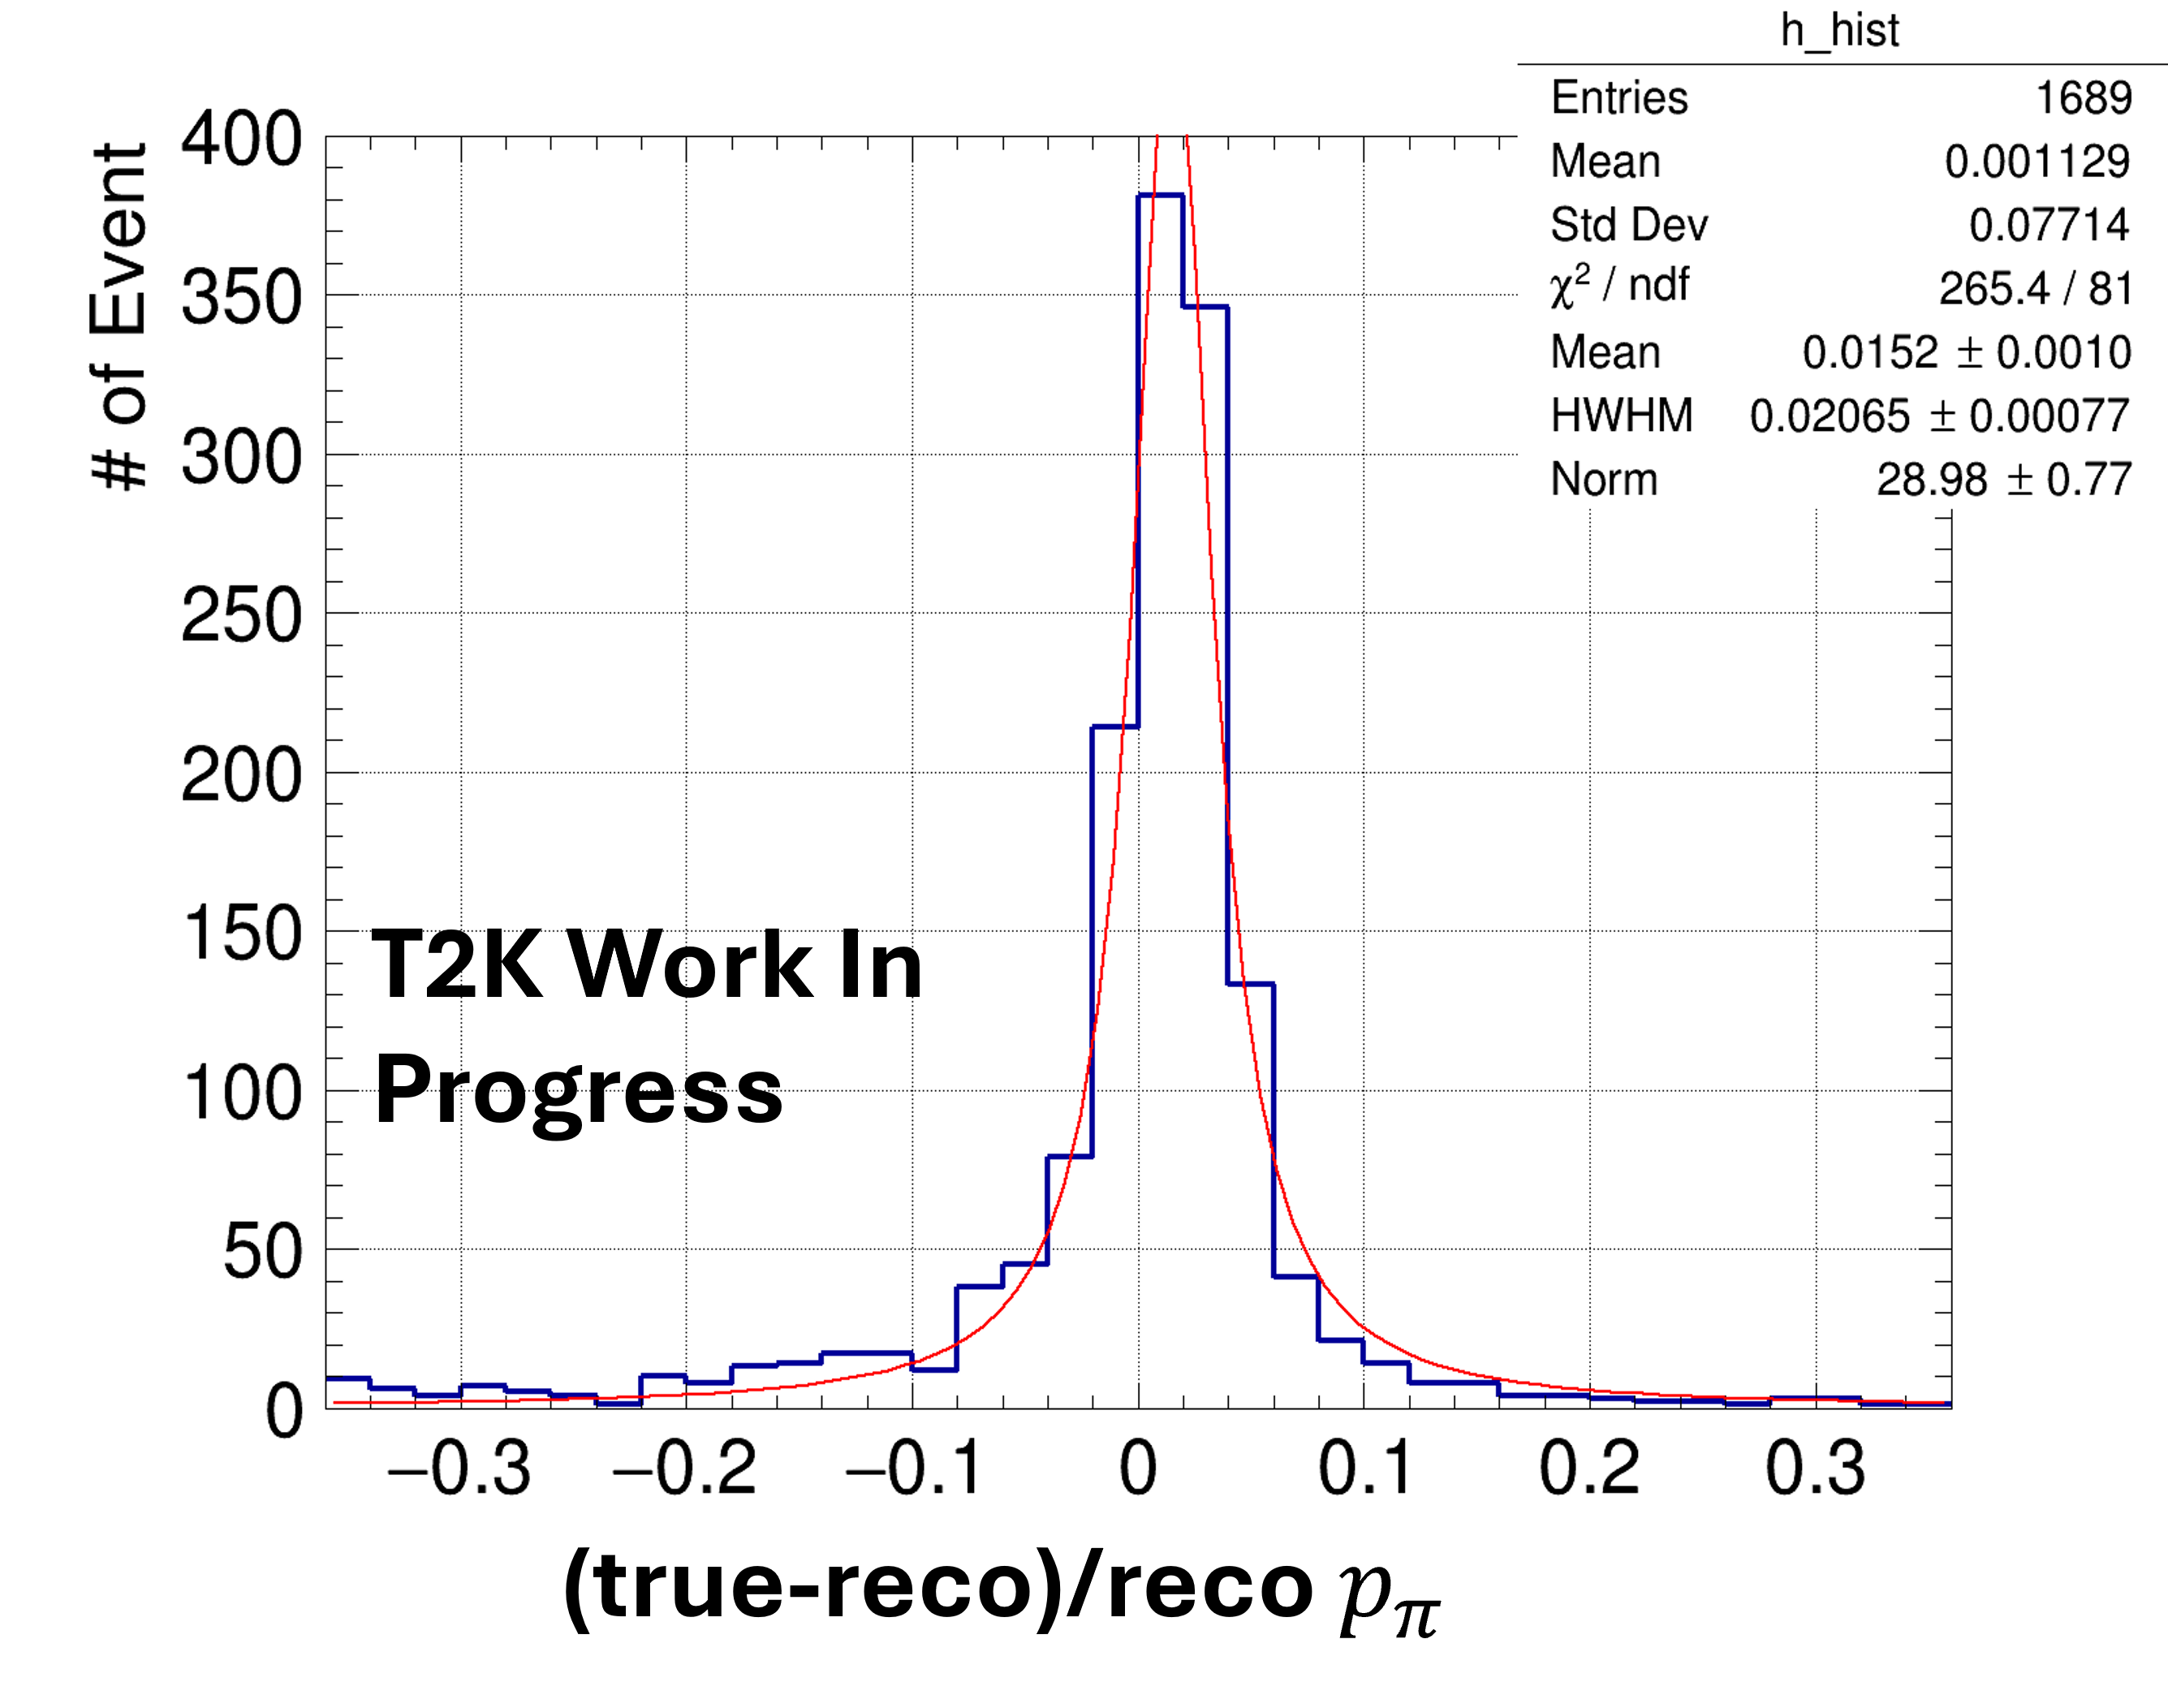
\includegraphics[width=\textwidth]{fig/ppi_res.png}
                    \caption{Momentum resolution.}
                    \label{fig:ppi-res}
               \end{subfigure}
               \begin{subfigure}{0.3\textwidth}
                    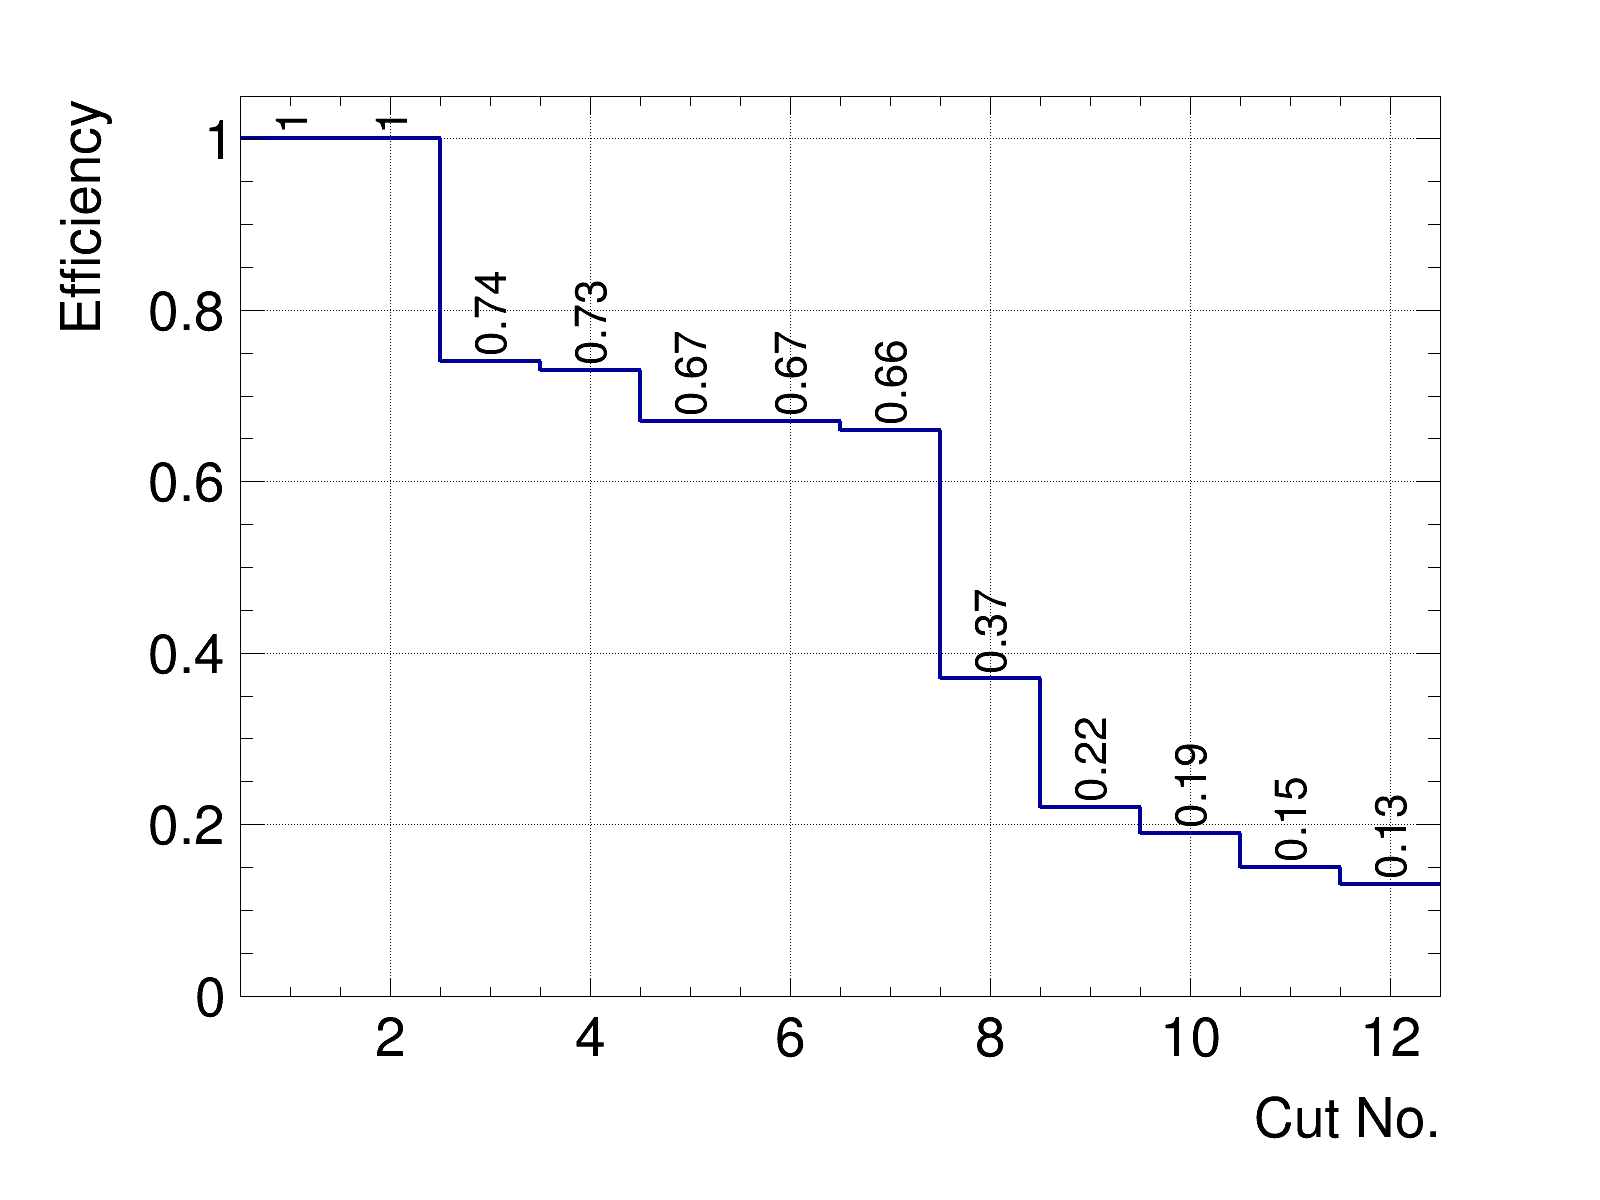
\includegraphics[width=\textwidth]{fig/INCL_p_pi_accum_eff_al11.png}
                    \caption{Accumulative efficiency.}
                    \label{fig:tl-accum-eff}
               \end{subfigure}
               \caption{Pion trackless reconstruction results.}
               \label{fig:piTLres}
            \end{figure}


            

    \subsection{Discussion}
        Both the pion and ESC proton selections are finished for muons going into the vertical TPC and SFGD. The High Angle TPC reconstruction is under development and will be expected to finish in the end of July 2024. Hence, the full selection will be done in the following months. The estimation of systematic uncertainties using control samples is being developed by colleagues and is expected to be done in the next few months. 


     \subsection{systematics ovaluation}
          